\section{Problem Formulation}
\begin{figure*}[!t]
\centering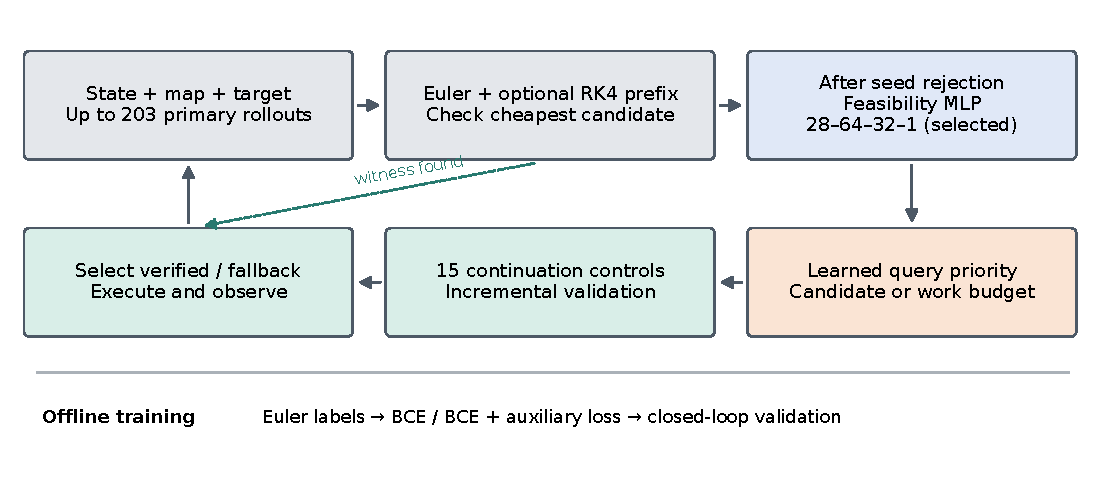
\includegraphics[width=.94\textwidth]{figures/architecture.pdf}
\caption{Local planning cycle. Terminal diversity schedules explicit continuation checks; a candidate-count or integration-step budget limits their work.}
\label{fig:architecture}
\end{figure*}

\subsection{Aircraft State and Local Planning}
The aircraft state is
\begin{equation}
 x=(p_x,p_y,h,V,\gamma,\psi,\phi,\alpha,T),
\end{equation}
where $h$ is altitude, $V$ is airspeed, $\gamma$ is flight-path angle, $\psi$ is heading, and $\phi$, $\alpha$, and $T$ are the roll, angle-of-attack, and specific-thrust actuator states. Each primitive holds the commanded input $u=(\phi_c,\alpha_c,T_c)$ constant for a duration $H$. First-order actuator dynamics maintain continuity across control switches. The model is given in Appendix~\ref{app:model}.

At a planning update, the primary library $\mathcal U_H(x_0)$ contains $N$ regularly sampled controls. Numerical integration produces a sampled trajectory $\tau_i=\Phi_H(x_0,u_i)$ and terminal state $x_i^+$. Let $\mathcal X$ denote the flight envelope, $\mathcal F$ the collision-free region after obstacle inflation, and $\mathcal O(x_0)$ the region available for validation at the current update. The primary feasibility indicator is
\begin{equation}
 A_i=\mathbf 1\{x\in\mathcal X,\ p(x)\in\mathcal F\cap\mathcal O(x_0)
                 \text{ for all }x\in\tau_i\}.
 \label{eq:primary}
\end{equation}
The principal experiments use the supplied obstacle map without a range restriction. A finite spherical $\mathcal O(x_0)$ is introduced in the range-limited diagnostic.

The primary task cost combines terminal distance, altitude error, terminal heading error, and command change:
\begin{align}
 J_i={}&w_d\|g-p_i^+\|+w_h|g_h-h_i^+|\nonumber\\
 &+w_\psi|\wrap(\psi_{g,i}-\psi_i^+)|
 +\|W_u(u_i-u_{\rm prev})\|_1 . \label{eq:cost}
\end{align}
Here $\psi_{g,i}$ points from the terminal position toward the target. The heading term is omitted within one meter of the horizontal target, and the command-change term is omitted before the first command. All methods use the same cost and primitive generator. If none of the regularly sampled primaries is feasible, they also test the preceding command over the full primary duration before declaring planning failure.

\subsection{Finite-Library Continuation Feasibility}
For each feasible primary, a terminal-dependent library $\mathcal B_B(x_i^+)$ contains $M$ continuation controls of duration $B$. The indicator
\begin{equation}
 C_i=\mathbf 1\left\{\begin{array}{l}\exists v\in\mathcal B_B(x_i^+),\ \forall x\in\Phi_B(x_i^+,v):\\
 x\in\mathcal X,\quad p(x)\in\mathcal F\cap\mathcal O(x_0)\end{array}\right\}
 \label{eq:continuation}
\end{equation}
uses the same sampled state and collision checks as~\eqref{eq:primary}. The continuation starts with the full terminal state, including actuator states; it does not restart at trim. Its observation boundary remains centered at the original planning state.

Full-library selection solves
\begin{equation}
 i^*=\arg\min_{i:A_i=1,\ C_i=1}J_i. \label{eq:full}
\end{equation}
The implementation checks continuation controls in a fixed order and stops checking a primary when it finds one feasible successor. The resulting pair is a finite continuation witness. When no witness is found within the available budget, the planner selects the cheapest feasible primary and records the unresolved continuation status. If the primary set is empty, the evaluation records a planning failure.

Two budgets are considered. A candidate budget $K$ limits the number of primary endpoints submitted for continuation validation. A work budget $W$ limits the total numerical integration steps spent on continuations. The latter accounts for rollouts that terminate early because of invalid dynamics. An unfinished rollout is never accepted as a complete witness. Primary propagation and schedule construction are included in elapsed planning time, but are reported separately from the continuation work budget.

\section{Maneuver-Diverse Validation}
\subsection{Terminal Representation and Physical Scaling}
For a feasible primary, the scheduling representation is $z_i=(\psi_i^+,h_i^+)$. Its two coordinates capture changes in turning direction and vertical maneuver. Let $V_0=\max(V_{\min},V(x_0))$ denote the airspeed used for scaling at the current update. Define the nominal scales
\begin{align}
 s_\psi&=\min\left(\pi,\frac{g\tan\phi_{\max}}{V_0}H\right),\\
 s_h&=V_0H\max(\tan\gamma_{\max},\tan|\gamma_{\min}|).
\end{align}
The distance between two terminal representations is
\begin{equation}
 d(i,j)^2=\left(\frac{\wrap(\psi_i^+-\psi_j^+)}{s_\psi}\right)^2
             +\left(\frac{h_i^+-h_j^+}{s_h}\right)^2. \label{eq:metric}
\end{equation}
Zero maneuver scales deactivate the corresponding coordinate. Circular heading differences avoid an artificial discontinuity at $\pm\pi$.

This representation is used only for scheduling. Every candidate is still validated in the full dynamic state. In particular, equal endpoint headings and heights do not imply equivalent velocity or actuator states. Physical scaling avoids a different problem: normalizing each coordinate by the observed candidate range can make millimeter-scale altitude differences dominate the selection when an altitude constraint compresses the candidate set.

\subsection{Cost-Seeded Farthest-First Schedule}
Let $\mathcal I=\{i:A_i=1\}$ and order this set stably by $J_i$. The schedule begins with the cheapest primary,
\begin{equation}
 s_1=\arg\min_{i\in\mathcal I}J_i.
\end{equation}
Subsequent candidates maximize their minimum distance to the selected set:
\begin{equation}
 s_{k+1}=\arg\max_{i\in\mathcal I\setminus S_k}
                       \min_{j\in S_k}d(i,j),\qquad
 S_k=\{s_1,\ldots,s_k\}. \label{eq:schedule}
\end{equation}
Ties are resolved by task cost and original library index. Under a candidate budget, the first $K$ scheduled endpoints are considered. Under a work budget, the schedule may contain all feasible primaries and validation stops when the integration allowance is consumed.

Among the scheduled primaries with a verified continuation, the algorithm selects the one with minimum $J_i$. It therefore uses diversity to distribute verification effort, not to replace the task objective. When the globally cheapest feasible primary passes the continuation test, selection can terminate immediately. Otherwise, the diversity schedule examines its remaining allowance because a later scheduled endpoint may have lower cost than an earlier verified endpoint. Cost-ordered validation terminates at its first witness, which is already the cheapest verified member of that ordered prefix.

\begin{algorithm}[t]
\caption{Budgeted terminal continuation selection}
\label{alg:search}
\begin{algorithmic}[1]
\Require State $x_0$, target $g$, primary library, budget $K$ or $W$
\State Propagate all primaries; retain feasible set $\mathcal I$
\If{$\mathcal I=\varnothing$}\State \Return planning failure\EndIf
\State Compute costs and schedule $S$ using~\eqref{eq:schedule}
\State $i_{\rm best}\gets\varnothing$, $w\gets0$
\For{each scheduled primary $i$ within the budget}
 \For{each continuation $v\in\mathcal B_B(x_i^+)$}
  \State Integrate with the remaining work allowance; update $w$
  \If{the complete continuation is feasible}
   \State Update $i_{\rm best}$ if $J_i$ improves its cost
   \State \textbf{break} the continuation loop
  \EndIf
  \If{the work allowance is exhausted}\State \textbf{break}\EndIf
 \EndFor
 \If{$i_{\rm best}$ is the cheapest feasible primary}\State \textbf{break}\EndIf
\EndFor
\If{$i_{\rm best}\ne\varnothing$}\State \Return primary and continuation witness
\Else\State \Return cheapest feasible primary and search status
\EndIf
\end{algorithmic}
\end{algorithm}

Maintaining the closest selected distance for each endpoint gives $O(NK)$ schedule construction for a $K$-candidate prefix. Primary propagation costs $O(NH/\Delta t)$. Continuation work scales as $O(KMB/\Delta t)$ in candidate-budget mode and is bounded by $W$ integration steps in work-budget mode. These operation counts expose an important distinction: the same number of checked primary endpoints need not entail the same amount of validation work.

\subsection{Incremental Constraint Rejection}
A continuation is feasible only if every sampled state satisfies its constraints. Once a sample violates a constraint, further integration cannot change the rejection. The incremental validator therefore terminates at the first violating sample and allocates the remaining work to subsequent controls or primary endpoints. A work-limit truncation is treated separately from a constraint rejection.

For a fixed candidate schedule without work truncation, this modification preserves the accepted continuation set and the selected primary. Both validators use the same deterministic integration prefix; a rejected prefix cannot become an accepted complete trajectory, while a feasible continuation is integrated to the same terminal sample. Under a hard work limit, the modification can change the decision by allowing the search to inspect more of the scheduled candidates. We compare complete-rollout and incremental-rejection validators on identical matched inputs.

\subsection{Search Status and Reuse Diagnostic}
The implementation distinguishes finding a witness, exhausting a budget, exhausting the finite continuation search, and having no feasible primary. Rejected continuations are classified by invalid dynamics, inflated-obstacle intersection, flight-envelope violation, and observation-boundary violation. Complete-rollout validation assigns reasons in this priority order. Incremental rejection records the first violating sample, resolving simultaneous violations by envelope, collision, and observation boundary; model-invalid states are rejected first. Truncation by a work limit is recorded separately.

An optional execution cache stores a previously verified primary--continuation pair. Elapsed execution removes time from this sequence, and reuse requires reintegration of its remaining segments from the current measured state. Revalidation produces a shrinking remaining trajectory, whereas a new primary--continuation pair restores the full planning durations. The main experiments disable this option to isolate scheduling. A separate diagnostic examines its interaction with a finite observation boundary and task progress.
